\section{Adjoint Sensitivity vs.\ Direct Autograd: Memory and Wall-Clock Cost}
\label{sec:track-a}

Two methods exist for computing gradients through a neural ODE. \textbf{Direct
autograd} treats the numerical integrator as an ordinary computational
graph: each of the solver's $N_t$ forward steps is recorded, and the reverse
pass walks back through every recorded step in turn, so peak memory grows
linearly with the number of steps taken. \textbf{Adjoint sensitivity}
\cite{chen2018neuralode} instead treats the forward solve as a black box and
derives a second, augmented ODE that produces the same gradient without
storing every intermediate state. Writing $\mathbf{a}(t) = \partial
L/\partial\mathbf{u}(t)$ for the adjoint state, it satisfies its own
backward-time differential equation,
\begin{equation}
\frac{d\mathbf{a}(t)}{dt} = -\mathbf{a}(t)^\top\frac{\partial \mathbf{f}_\theta}{\partial\mathbf{u}}(\mathbf{u}(t)),
\qquad
\frac{dL}{d\theta} = \int_{t_1}^{t_0}\mathbf{a}(t)^\top\frac{\partial\mathbf{f}_\theta}{\partial\theta}(\mathbf{u}(t))\,dt,
\label{eq:adjoint}
\end{equation}
solved backward from $t_1$ to $t_0$ alongside the original state
$\mathbf{u}(t)$ (recomputed rather than stored), so memory depends only on
the size of the state and parameter vectors, not on how many steps the
forward solve took -- an $O(1)$ memory cost in trajectory length, against
direct autograd's $O(N_t)$. This project's own implementation documentation
adopts direct autograd on the stated grounds that this $O(1)$ advantage does
not matter for this project's short trajectories ($N_t\in[36,101]$). This
section measures that claim directly on an RTX~3060, holding the integrator
fixed (classical RK4 at matched step size on both paths; a forward-trajectory
check confirms the two implementations agree to $\sim10^{-7}$ relative
error) so that only the differentiation method varies.

\begin{expectbox}
\expectrow{Question}{Does adjoint sensitivity's constant memory cost make it the better choice at this project's trajectory lengths, as the project's own documentation assumes?}
\expectrow{Expected}{Direct autograd should be cheaper in memory at these short lengths, with adjoint's advantage only appearing once trajectories grow much longer.}
\expectrow{Observed}{Adjoint already uses less memory at every length tested. The deciding cost is wall-clock, not memory: adjoint is $1.9$--$2.1\times$ slower.}
\end{expectbox}

\begin{table}[!ht]
\centering
\small
\renewcommand{\arraystretch}{1.15}
\caption{Peak VRAM and wall-clock, direct autograd vs.\ adjoint sensitivity.}
\label{tab:adjoint-profiling}
\begin{tabularx}{\textwidth}{@{}X C{1.2cm} L{3.0cm} C{2.4cm} C{2.6cm}@{}}
\toprule
\hdrrow \thh{System} & \thh{Trajectory length $N_t$} & \thh{Method} & \thh{Peak VRAM (MB)} & \thh{Seconds per 1000 epochs}\\
\midrule
Lotka-Volterra & 36 & Direct autograd & 18.61 & 317.5\\
Lotka-Volterra & 36 & Adjoint & 17.08 & 672.9\\
SIR & 101 & Direct autograd & 21.52 & 984.8\\
SIR & 101 & Adjoint & 17.12 & 1871.6\\
\bottomrule
\end{tabularx}
\end{table}

\begin{figure}[htbp]
\centering
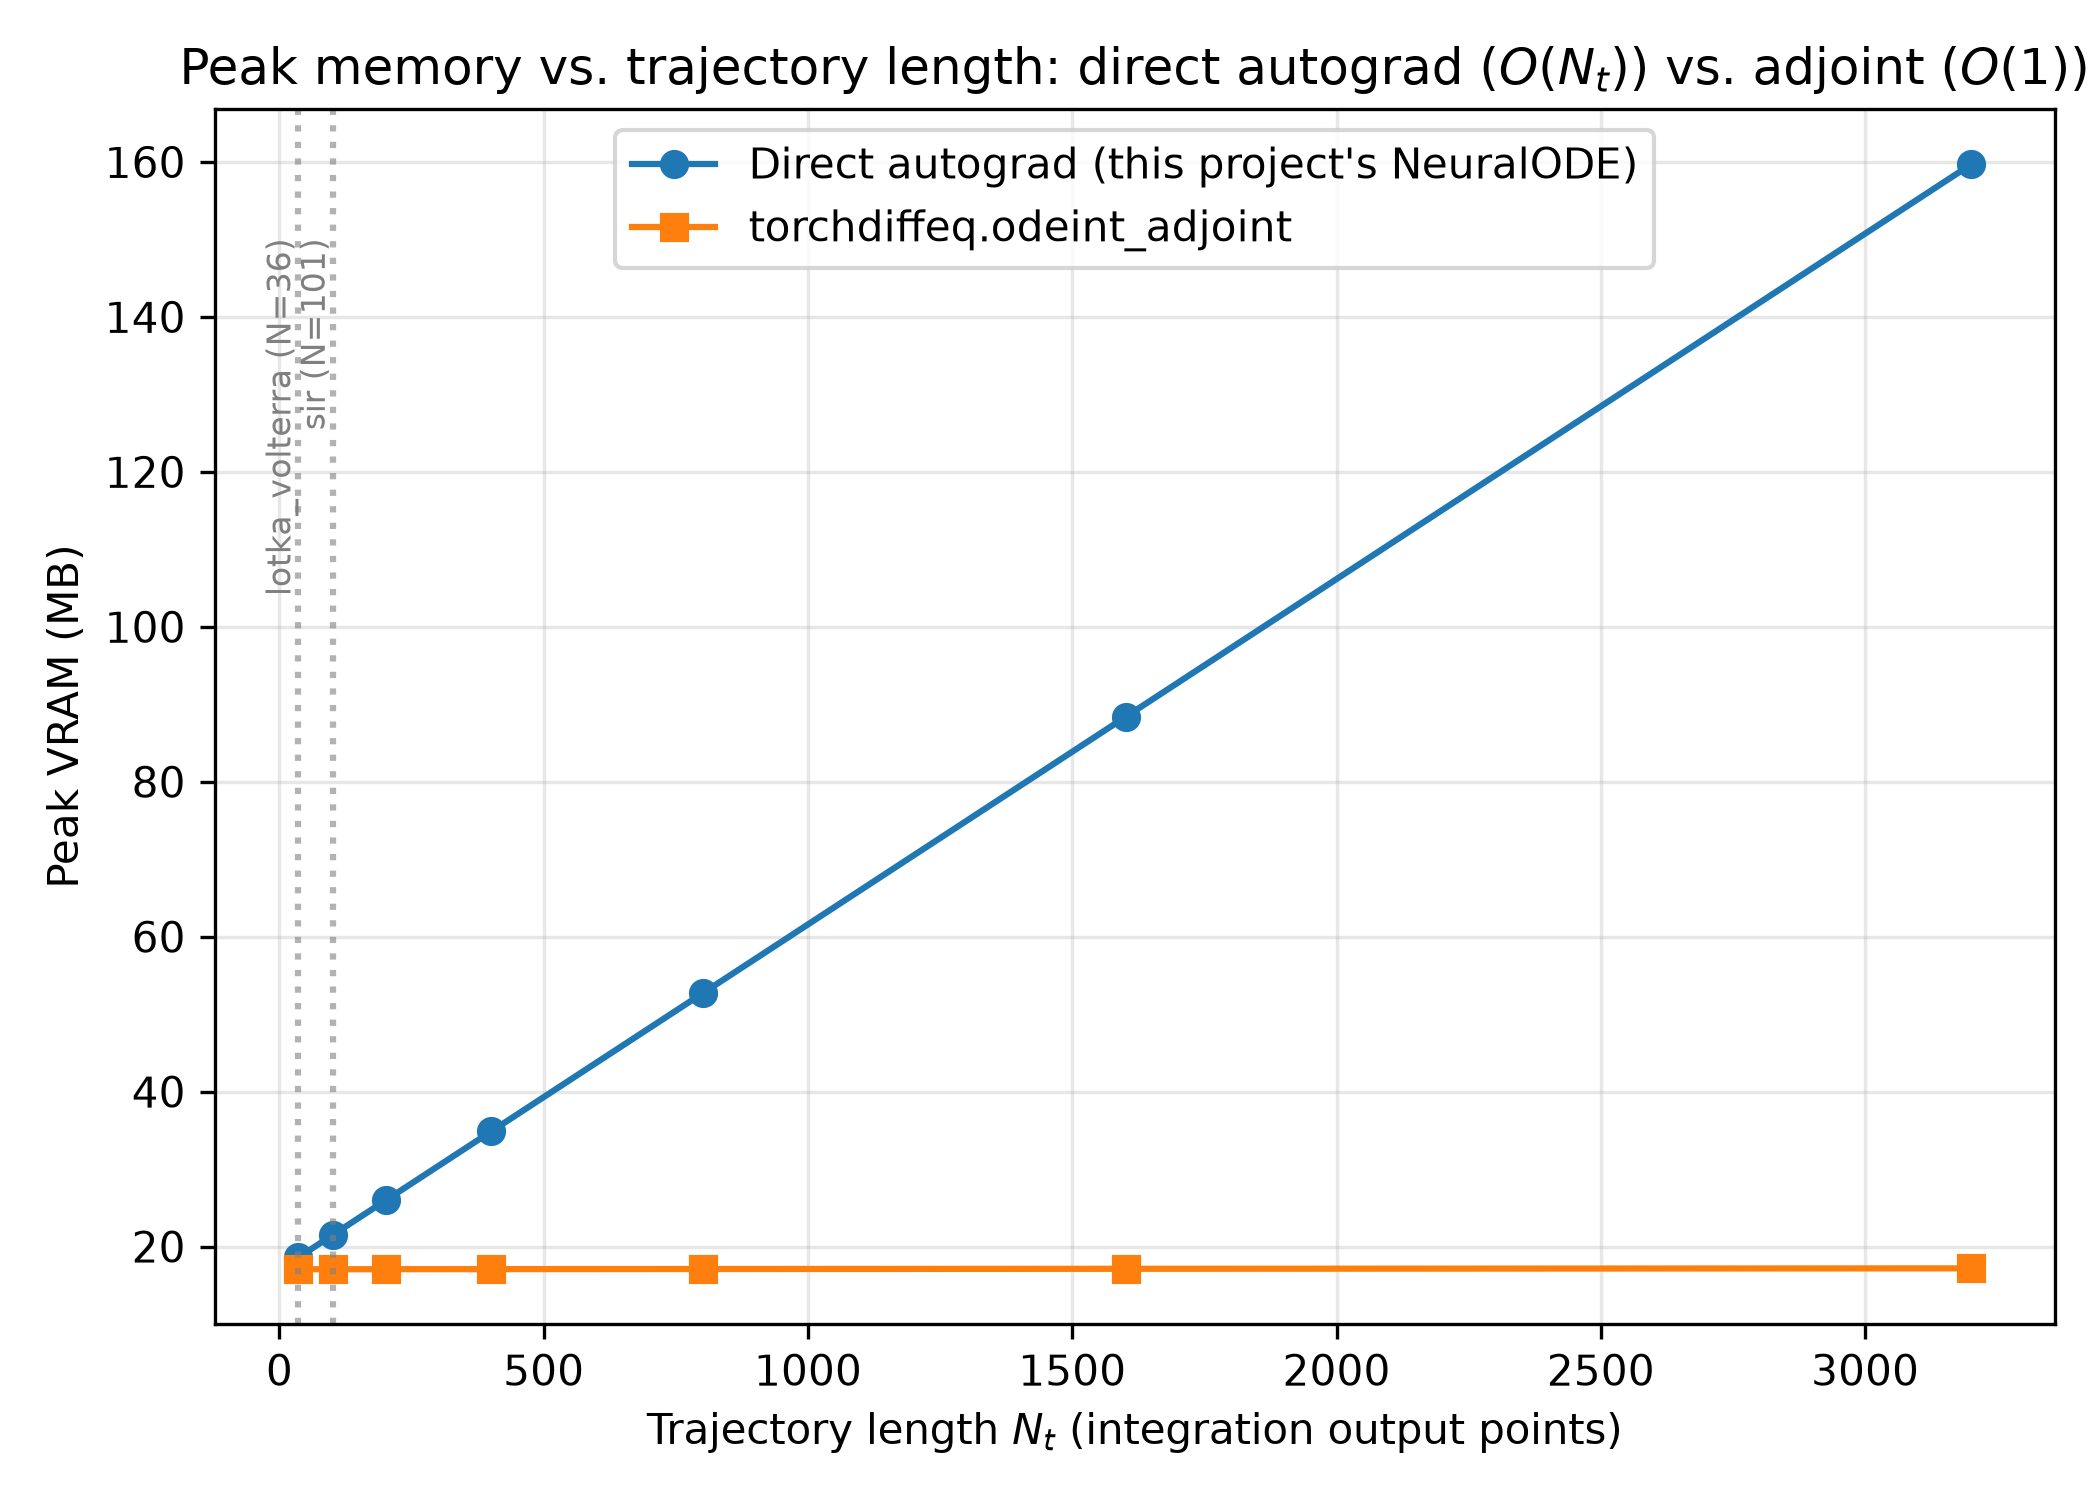
\includegraphics[width=0.75\linewidth]{figures/track_a/memory_vs_trajectory_length.png}
\caption{Peak memory vs.\ trajectory length $N_t\in\{36,\dots,3201\}$: direct
autograd grows linearly ($\approx0.045$~MB per output point); adjoint stays
flat (0.7\% increase over an $89\times$ length increase).}
\label{fig:adjoint-memory}
\end{figure}

\paragraph{Finding.} The measured memory data contradicts the stated
premise behind the original choice, while still supporting its conclusion.
The $O(N_t)$ vs.\ $O(1)$ scaling in Equation~\ref{eq:adjoint} predicts a
crossover length below which direct autograd's smaller constant factor
should still win on raw memory, since it avoids the adjoint method's own
bookkeeping overhead; the data shows no such crossover inside the tested
range. Adjoint uses \emph{less} memory than direct autograd at every tested
length, including the shortest ($N_t=36$: $17.08$ vs.\ $18.61$~MB) --
Figure~\ref{fig:adjoint-memory} shows direct autograd's per-step storage cost
is already large enough at this project's scale to outweigh whatever
constant overhead the adjoint method's own bookkeeping carries.
Extrapolating the measured linear slope of direct autograd's memory growth,
$N_t$ would need to reach $\approx225{,}000$ before it threatens a 12~GB
card. The deciding factor for
this project is wall-clock: solving the continuous adjoint ODE backward in
time costs a consistent $1.9$--$2.1\times$ overhead at both tested lengths,
turning a 53-minute Lotka-Volterra run into $\sim$112~minutes for a memory
saving that never becomes load-bearing (peak usage is $0.17\%$ of card
capacity). Gradient relative error is $2.85\times10^{-7}$ and
$4.88\times10^{-7}$ respectively, well inside a $5\times10^{-3}$ tolerance --
both methods agree numerically, so the choice reduces to a resource
trade-off. Direct autograd is the faster option for every dataset in this
project's scope ($N_t\le201$).

\FloatBarrier
